\documentclass{note}
\usepackage[cpp,table,pseudo]{mypackage}
\usepackage{footnote}
\usepackage{forest}
\makesavenoteenv{tabular}
\usetikzlibrary{automata,backgrounds,fit,shapes,positioning}

\tikzset{->, % makes the edges directed
>=stealth, % makes the arrow heads bold
node distance=2cm, % specifies the minimum distance between two nodes. Change if necessary.
every state/.style={thick, fill=gray!10}, % sets the properties for each 'state' node
}

\renewcommand{\thefootnote}{\fnsymbol{footnote}}

\title{编译原理笔记}
\author{陈鸿峥}
\date{{\builddatemonth\today}\protect\footnote{\text{Build \builddate\today}}} % protect!

\begin{document}

\maketitle
\renewcommand{\thefootnote}{\arabic{footnote}}
\setcounter{footnote}{0}

\setcounter{tocdepth}{2}%设置深度
\tableofcontents

\bigskip\bigskip

% !TEX root = main.tex

\section{计算机系统概述}
\subsection{计算模型}
\begin{itemize}
	\item 图灵机(1936)
	\item 冯诺依曼体系结构(1945)\footnote{非冯诺依曼体系结构:并行计算、量子计算、生物计算} --- 存储程序原理(\textbf{运算器}为中心)\\
	计算机采用\textbf{二进制}表示机器指令和数据,按照程序指令\textbf{顺序}执行
\begin{center}
\begin{tikzcd}
& & \text{存储器}\arrow{d} & & \\
\quad\arrow{r} & \text{输入设备}\arrow{r} & \text{运算器}\arrow{r}\arrow{d}\arrow{u} & \text{输出设备}\arrow{r} & \quad\\
& & \text{控制器}\arrow{u}\arrow{lu}\arrow{ru}\arrow[bend left]{uu} & &
\end{tikzcd}
\end{center}
而现在由于计算不是瓶颈,存储访问成为了瓶颈,故现代微机以\textbf{存储器}为中心
\begin{center}
\begin{tikzcd}
& & \text{运算器}\arrow{d} & & \\
\quad\arrow{r} & \text{输入设备}\arrow{r} & \text{存储器}\arrow{r}\arrow{d}\arrow{u} & \text{输出设备}\arrow{r} & \quad\\
& & \text{控制器}\arrow{u}\arrow{lu}\arrow{ru}\arrow[bend left]{uu} & &
\end{tikzcd}
\end{center}
\end{itemize}
[运算器、控制器](CPU)、存储器为计算机的核心,合称主机;外围设备,简称外设,指除主机外的其他设备,包括IO设备、外存等

计算机中的信息仍用二进制表示的原因:由物理器件性能决定
\begin{itemize}
	\item 二进制只有两种状态,容易找到具有2个稳定状态并且状态转换容易控制的物理器件(数字电路)
	\item 二进制编码运算规则简单
	\item 二进制的0、1与二值逻辑一致,容易实现逻辑运算
\end{itemize}
% There are two reasons computers use the binary system:
% 1.Two clearly distinct states that provide a safety range for reliability.
% 2.Least amount of necessary circuitry, which results in the least amount of space, energy consumption, and cost.

\subsection{计算机的发展历程}
按发展历程可分为:电子管、晶体管、集成电路、(超)大规模集成电路四代计算机
\par重大历史事件如下
\begin{center}
\begin{tabular}{|c|c|c|c|}
\hline
% 年份 & 姓名 & 事件 & 备注 \\
1904 & 弗莱明(Fleming) & 二极管 & \\\hline
1907 & 德福雷斯特(De Forest) & 三极管 & \\\hline
1938 & 香农(Shannon) & 布尔代数与二值电子器件(继电器) & 奠定数字电路基石 \\\hline
1946 & & 第一台通用计算机ENIAC & 十进制 \\\hline
1947 & \begin{tabular}{c}布莱顿(Brattain)\\
巴丁(Bardeen)\end{tabular} & 点接触晶体管 & \\\hline
1949 & 肖克利(Shockley) & 结型晶体管(1949) & 1956诺贝尔奖\\\hline
1950 & & 二进制和存储程序EDVAC & 实现冯诺依曼设想(组合进步) \\\hline
1958 & Jack Kilby & 集成电路 & 2000诺贝尔奖 \\\hline
1965 & Moore & 摩尔定律 & \begin{tabular}{c}
在价格不变的情况下,每18个月芯片上\\
晶体管数目翻倍,性能也提升一倍
\end{tabular}\\\hline
1971 & Intel & 第一款微处理器4004 & 10$\mu$m\\\hline
\end{tabular}
\end{center}

\subsubsection{单处理器(1971-2002)}
性能提升主要手段
\begin{itemize}
	\item 提升工作主频:KHz增长至GHz(生产工艺进步,流水线级数增加)
	\item 指令级并行(ILP)
\end{itemize}
\begin{proposition}[安迪-比尔定律]
Andy gives, Bill takes away. 安迪是原Intel CEO,比尔是原微软CEO,硬件厂商靠软件开发商用光自己提供的硬件资源得以生存
\end{proposition}
但遇到频率墙和功耗墙
\[\text{功耗(power)}\propto 1/2\times\text{CMOS电容}\times\text{电压}^2\times\text{转换(01)频率}\]
\par
2004年,Intel放弃4GHz Pentium4芯片开发,因无法解决散热问题,通过加快主频提升处理器性能的路走到尽头

\subsubsection{多核处理器(2005-)}
采用多核处理器不过是将硬件的问题丢到软件\footnote{“向多核的转变并不是因为我们在软件或体系结构技术上取得了中大突破而带来的。相反,这种转变是当单处理器体系结构发展遇到了难以克服的巨大障碍时,我们被迫作出的一种选择。”---Kurt Keutzer (UCB), \emph{The Landscape of Parallel Computing Research: A View from Berkeley}}
\begin{theorem}[阿姆达尔(Amdahl)定律]
\label{thm:amdahl}
\[\text{改进后的执行时间}=\text{受改进影响部分的执行时间}/\text{改进提高的倍数}+\text{不受影响的执行时间}\]
\[S_A=\frac{1}{s+(1-s)/N},\]
\end{theorem}
对计算机系统的某个部分采用并行优化措施后所获得的计算机性能的提高是有上限的,上限由串行部分所占的比例决定
\begin{theorem}[古斯塔夫森(Gustafson)定律]
\[S_G=(s'+p'\times N)/(s'+p')=N+(1-N)\times s',\]
其中,$s'$和$p'$为程序串行部分与可并行化部分在并行系统上执行的时间占总时间的比例,$N$为处理器数量,简便起见设总时间$s'+p'=1$
\end{theorem}
打破Amdahl定律\textbf{问题规模不变}的假设,任何足够大的任务都可以被有效地并行化,只要问题规模可扩展,并行所带来的加速比就可以扩展


\subsection{计算机系统的层次结构}
\begin{center}
\begin{tikzcd}
\text{高级语言层}\arrow{d}{}\\
\text{汇编语言层}\arrow{d}{}\\
\text{操作系统层}\arrow{d}{}\\
\text{指令系统层}\arrow{d}{}\\
\text{微体系结构层}\arrow{d}{}\\
\text{数字逻辑层}
\end{tikzcd}
\end{center}
程序编译运行过程:
\begin{center}
\begin{tikzcd}
\text{高级语言}\quad\arrow{r}{\text{预编译、编译}} & \quad\text{汇编语言}\arrow{r}{\text{汇编}} & \text{目标文件(二进制)}\arrow{r}{\text{链接}} & \text{可执行文件(二进制)}\arrow{d}{\text{加载}}\\
& & \text{电路上的电信号}\quad & \quad\text{二进制机器指令流(硬盘$\to$存储器)}\arrow[swap]{l}{\text{CPU取指译码}}
\end{tikzcd}
\end{center}
计算机内部工作过程:逐条执行加载到内存中的二进制机器指令流的过程

指令执行分为两个阶段,周期性重复性进行:
\begin{itemize}
	\item 取指阶段:CPU从内存中读取指令,程序计数器(PC)保存要被要被取出的\textbf{下一条}指令的地址,除非遇跳转指令,否则都加一个增量\footnote{程序计数器(Program Counter)是一个实际存在的寄存器吗? - Belleve的回答 - 知乎 \url{https://www.zhihu.com/question/22609253/answer/21965180} PC每次增加\textbf{一条指令的长度/寻址粒度},在MIPS中一条指令长4字节,寻址粒度1字节,故每次PC加4;而x86体系指令长度不定,每次增加量会变化}
	\item 执行阶段:对取出的指令译码后执行
\end{itemize}
软件系统可分为系统软件和应用软件

\subsection{计算机结构的八个想法}
\begin{enumerate}
	\item 摩尔(Moore)定律:集成电路资源每$18-24$个月翻倍
	\item 抽象(abstraction):简化设计
	\item 加速常用操作(Make common case fast):见定理\ref{thm:amdahl}
	\item 并行(parallelism)
	\item 流水线(pipelining)
	\item 预测(prediction)
	\item 内存等级制(hierarchy)
	\item 冗余实现可靠性(redundancy):检测故障及解决
\end{enumerate}

\subsection{基本指标}
表示计算机通信带宽时
\begin{center}
\begin{tabular}{ccccccc}\hline
KB(yte) & MB & GB & TB & PB & EB & ZB\\\hline
$10^3$ & $10^6$ & $10^9$ & $10^{12}$ & $10^{15}$ & $10^{18}$ & $10^{21}$\\\hline
\end{tabular}
\end{center}
表示计算机存储二进制时
\begin{center}
\begin{tabular}{ccccccc}\hline
KiB(yte) & MiB & GiB & TiB\\\hline
$2^{10}$ & $2^{20}$ & $2^{30}$ & $2^{40}$\\\hline
\end{tabular}
\end{center}
\begin{itemize}
	\item 位(bit/b):计算机处理、存储、传输信息的最小单位
	\item 字节(Byte/B) $1\text{ Byte}=8\text{ bit}$:现代计算机主存按字节编制,字节是最小可寻址单位
	\item 字(Word):表示被处理信息的单位,用来度量数据类型的宽度\footnote{字长是指CPU中\textbf{数据通路的宽度},等于CPU内部总线的宽度或运算器的位数或通用寄存器的宽度;字和字长的宽度可以一样,也可以不同,通常是字节的整数倍}
\end{itemize}
\par 一台32位的电脑,一个字等于4个字节,字长为32位;若字长为16位,则一个字等于2字节.
\par 4字节相当于8位16进制编码

\subsection{性能评价}
\label{subsec:performance}
CPU主频:对同一型号计算机,主频越高,完成指令一个执行步骤时间越短
\[\text{计算机的性能(Performance)}=1/\text{执行时间(Execution time)}\]
按照单位(量纲)进行换算即可
\[\begin{aligned}
\text{CPU执行时间(s)}&=\text{执行程序所需CPU时钟周期(cyc)}\times\text{时钟周期s/cyc)}\\
&=\text{指令数目(ins)}\times\text{CPI(cyc/ins)}\times\text{时钟周期(s/cyc)}
\end{aligned}\]
程序性能对执行事件的影响:
\begin{center}
\begin{tabular}{|c|c|c|c|}\hline
 & 指令数 & CPI & 时钟周期\\\hline
算法、编程语言、编译器 & $\times$ & $\times$ & \\\hline
指令集 & $\times$ & $\times$ & $\times$ \\\hline
计算机组成 & & $\times$ & $\times$ \\\hline
实现技术 & & & $\times$\\\hline
\end{tabular}
\end{center}
体系结构=指令集体系结构(功能定义与设计)+计算机组成(考虑用什么材料)\\
举例来说:
\begin{itemize}
	\item 指令集(ISA)考虑:是否提供乘法指令
	\item 组成(Organization)考虑:如何实现乘法指令(专门乘法器还是加法器+移位器)
	\item 实现技术(Technology)考虑:如何布线、用什么材料和工艺
\end{itemize}

% 带有处理器的设备一般称为智能化设备
% 完整的计算机系统应包括配套的硬件设备和软件系统
% !TEX root = main.tex

\section{词法分析}
分离词法分析和语法分析可以简化这两个任务,同时提升编译器的性能与兼容性。

\subsection{基本定义}
\begin{definition}
令牌(token)是一个\underline{令牌名字}与\underline{可选属性值}构成的对;模式(pattern)描述了每个词素(lexeme)要遵循什么规则;而词素(最小意义单位)则是源程序中一连串满足模式的字母,作为令牌的实例化。
\end{definition}
\begin{example}
考虑C语句\\
 \qquad\qquad\verb'printf("Total = %d\n", score);'\\
其中\verb'printf'和\verb'score'是匹配(match)上令牌\textbf{id}模式的词素,而\verb'"Total = %d\n"'是匹配上字面值\textbf{literal}的词素。
\end{example}
简单来讲,令牌是一个更大的概念,是同类词素的集合。
比如一个令牌\textbf{comparison}的样例词素可以有\texttt{<=}和\texttt{!=}。

\begin{definition}[字母表与语言]
字母表(alphabet)$\Sigma$是有限符号(symbol)的集合,如ASCII就是一个字母表。
字符串(string)$s$是从字母表中抽取的有限符号的序列,$|s|$为字符串长度,$\epsilon$为空串。
语言(language)是字符串的可数集合。
\end{definition}
\begin{example}
字母表$\Sigma=\{0,1\}$,则$\{001,1001\}$和$\{\}$都是定义在$\Sigma$上的语言。
\end{example}

语言是一种集合,故集合运算也适用于语言。
\begin{table}[H]
\centering
\begin{tabular}{|c|c|}\hline
并集(union) & $L\cup M$\\\hline
连接(concatenation)/交集 & $LM$\\\hline
柯林闭包(Kleene closure) & $L^*=\cup_{i=0}^\infty L^i$\\\hline
正闭包(positive) & $L^+=\cup_{i=1}^\infty L^i$\\\hline
\end{tabular}
\end{table}

\subsection{正则表达式}
\begin{definition}[正则表达式(regular expression, regex)]
正则表达式$r$定义了语言$L(r)$,以递归形式定义:
\begin{enumerate}
	\item 奠基:
	\begin{itemize}
		\item $\epsilon$是正则表达式,即$L(\epsilon)=\{\epsilon\}$
		\item $a\in\Sigma$是正则表达式,即$L(\va)=\{a\}$(这里用斜体代表符号,粗体代表符号对应的正则表达式)
	\end{itemize}
	\item 推论:若$r$和$s$都是正则表达式给出了语言$L(r)$和$L(s)$,则
	\begin{itemize}
		\item $(r)|(s)$是正则表达式,表示$L(r)\cup L(s)$
		\item $(r)(s)$是正则表达式,表示$L(r)L(s)$
		\item $(r)^*$是正则表达式,表示$(L(r))^*$
		\item $(r)$是正则表达式,表示$L(r)$
	\end{itemize}
\end{enumerate}
正则表达式表示的语言叫做正规集。
\end{definition}

有以下运算规定:
\begin{itemize}
	\item 一元运算符${}^*$有最高优先级,左结合
	\item 连接优先级次之,左结合
	\item $|$优先级\textbf{最低},左结合
\end{itemize}

\begin{definition}[正则定义]
$d_i\to r_i$,其中$d_i$都是名字,且各不相同。
每个$r_i$是$\Sigma\cup\{d_1,\ldots,d_{i-1}\}$中符号上的正则表达式。
\end{definition}
\begin{example}
比如C语言的标识符可记为
\[\begin{aligned}
letter\_ &\to A|B|\cdots|Z|a|b|\cdots|z|\_\\
digit &\to 0|1|\cdots|9\\
id &\to letter\_(letter\_|digit)^*
\end{aligned}\]
\end{example}

正则表达式的拓展\footnote{更多可参见\href{https://regex101.com/}{Regex101}}:
\begin{itemize}
	\item $r^+$代表一个或多个
	\item $r?$代表零或一个
	\item $[a-z]$字母类
\end{itemize}
% !TEX root = main.tex

\section{语法分析}
\subsection{上下文无关文法}
语法分析需要解决:从词法分析中获得的每个属性字(token)在语句中承担什么角色,同时检查语句是否符合程序语言的语法。

很多语言并非是正则的,比如匹配的括号串$\{(^i)^i\mid i\geq 0\}$,原因是FA不能记住其访问某一状态的次数,因此需要有更加强大的语言。

\subsubsection{基本定义}
\begin{definition}[上下文无关文法(context-free gramma, CFG)]
包括四部分
\begin{itemize}
	\item 终端符号(terminal)的集合$T$(即token名字)
	\item 非终端符号的集合$N$
	\item \textbf{唯一的}开始符号$S\in N$
	\item 若干以下形式的产生式(production)
	\[X\to Y_1Y_2\ldots Y_n\]
	其中$X\in N$且$Y_i\in T\cup N\cup\{\epsilon\}$。
	多个\textbf{左侧相同}的产生式右侧可用$\mid$合并。
\end{itemize}
\end{definition}
\begin{definition}[推导(derivation)]
从开始符号开始,每一步推导就是用一个产生式的右方取代左端的非终端符号。
\end{definition}

CFG定义语言的能力比正则表达式强很大原因是它引入了\textcolor{red}{\textbf{递归}}的因素。

\begin{example}
用上下文无关文法定义下列语言:
\begin{itemize}
	\item $L=\{0^n1^n\mid n\geq 1\}$:$E\to 0E1\mid 01$
	\item 只含有$0$和$1$的回文串:$S\to 0S0\mid 1S1\mid 0\mid 1\mid \epsilon$
	\item 只含有$($和$)$的匹配括号串:$E\to (E)\mid EE\mid \epsilon$
\end{itemize}
\end{example}

\begin{itemize}
	\item 最左推导(left-most):每步推导都替换最左侧的非终端符号
	\[E\xRightarrow{lm}
	-E\xRightarrow{lm}
	-(E)\xRightarrow{lm}
	-(E+E)\xRightarrow{lm}
	-(id+E)\xRightarrow{lm}
	-(id+id)\]
	\item 最右推导(right-most):每步推导都替换最右侧的非终端符号
	\[E\xRightarrow{rm}
	-E\xRightarrow{rm}
	-(E)\xRightarrow{rm}
	-(E+E)\xRightarrow{rm}
	-(E+id)\xRightarrow{rm}
	-(id+id)\]
\end{itemize}

\begin{definition}[二义性]
如果对于一个文法,存在一个句子,对这个句子可以构造两棵不同的分析树,那么我们称这个文法为二义的。
\end{definition}
看语法分析树的叶子结点能不能连成句子。

\begin{example}
对于文法$E\to E+E\mid E*E\mid -E\mid (E)\mid id$及句子$id+id*id$,有以下两种推导:

\begin{minipage}{0.5\linewidth}
\[\begin{aligned}
E &\implies E+E\\
&\implies id+E\\
&\implies id+E*E\\
&\implies id+id*E\\
&\implies id+id*id
\end{aligned}\]
\end{minipage}
\begin{minipage}{0.5\linewidth}
\[\begin{aligned}
E &\implies E*E\\
&\implies E+E*E\\
&\implies id+E*E\\
&\implies id+id*E\\
&\implies id+id*id
\end{aligned}\]
\end{minipage}
\end{example}

文法二义性可通过引入更多的产生式来消除。
\begin{example}
$E\to E+E\mid E*E\mid (E)\mid id$是有二义的,因为不知道应该先算加法还是乘法。
可将其改为
\[\begin{aligned}
E &\to E+T\mid T\\
T &\to T*F\mid F\\
F &\to (E)\mid id
\end{aligned}\]
其中$E$为Expression,$T$为Term,$F$为Factor,即可消除二义性(必然得先算乘法)。
相当于先算$F$,再算$T$,最后算$E$,强行添加了括号/优先级。
\end{example}
\begin{example}[悬挂的if-else]
\verb'if E1 then if E2 then E3 else E4',可以令\verb'else'匹配最近的\verb'then'。
\[\begin{array}{rll}
E &\to MIF &\text{// 所有的then都被匹配}\\
  &\mid UIF &\text{// 仅有一些then}\\
MIF &\to \text{if } E \text{ then } MIF \text{ else } MIF &\\
  &\mid OTHER &\\
UIF &\to \text{if } E \text{ then } E &\\
  &\mid \text{if } E \text{ then } MIF \text{ else } UIF &
\end{array}\]
\end{example}

并不是所有上下文无关文法都可以做到无二义,也无法判断一个上下文无关文法是否是二义的。

\subsubsection{NFA转CFG}
\begin{enumerate}
	\item 对于NFA的每一状态$i$,创建非终态$A_i$
	\item 若状态$i$在输入$a$上有转换边到状态$j$,则添加生成式$A_i\to aA_j$;
	若状态$i$在输入$\epsilon$上转换到状态$j$,则添加生成时$A_i\to A_j$
	\item 若$i$是接受状态,则添加$A_i\to\epsilon$
	\item 若$i$是初始状态,则令$A_i$为语法的初始符号
\end{enumerate}

\begin{definition}[右线性文法]
如果每个产生式都属于下列形式之一
\[A\to aB\qquad A\to a\qquad A\to\epsilon\]
则这样的文法称为右线性文法
\end{definition}
\begin{definition}[左线性文法]
如果每个产生式都属于下列形式之一
\[A\to Ba\qquad A\to a\qquad A\to\epsilon\]
则这样的文法称为左线性文法
\end{definition}
\begin{theorem}
正则表达式/NFA/DFA与左/右线性文法得表达能力是等价的
\end{theorem}

在处理程序时,上下文无法文法存在局限性,无法解决诸如以下问题:
\begin{itemize}
\item 变量先声明,再使用
\item 调用函数时,实参个数和形参个数一致
\end{itemize}
都得留到语义分析阶段才解决。

\subsection{基础概念与处理}
对于CFG的预处理包括\textbf{消除左递归}和\textbf{提取左因子}。

\subsubsection{消除左递归}
\begin{definition}[左递归]
对于非终端符号$A$有生成式$A\to A\alpha$,则该文法是左递归的。
\end{definition}

消除左递归的方法:先把单元素拎出来放左侧,然后把所有递归移至右侧
\[A\to A\alpha_1\mid \cdots\mid A\alpha_m\mid\beta_1\mid\cdots\beta_n
\implies
\begin{aligned}
A &\to\beta_1 A'\mid\cdots\mid\beta_n A'\\
A' &\to\alpha_1 A'\mid\cdots\mid\alpha_m A'\mid\textcolor{red}{\epsilon}
\end{aligned}\]

\begin{example}
如果是多级左递归,则需要先将上级生成式代入到中间级生成式中,再做消除。
如下例
\[\begin{aligned}
S &\to Aa\mid b\\
A &\to Ac\mid Sd\mid \epsilon
\end{aligned}\]
将下式改写为$A \to Ac\mid Aad\mid bd\mid \epsilon$,进而可消除左递归
\[\begin{aligned}
S &\to Aa\mid b\\
A &\to bdA'\mid A'\\
A' &\to cA'\mid adA'\mid \epsilon
\end{aligned}\]
\end{example}

\subsubsection{提取左因子}
\begin{definition}[提取左因子(left-factoring)]
将生成式右侧左部相同的因子部分提取出来,找最长前缀
\[A\to\alpha\beta_1\mid\alpha\beta_2\mid\cdots\alpha\beta_n\mid\gamma\]
$\gamma$代表所有不以$\alpha$开始的生成式,提取左因子则得到(将$\alpha$拿出来)
\[\begin{aligned}
A &\to \alpha A'\mid\gamma\\
A' &\to \beta_1\mid\beta_2\mid\cdots\beta_n
\end{aligned}\]
直至没有生成式有相同前缀
\end{definition}

\subsubsection{FIRST集与FOLLOW集}
\begin{definition}[FIRST集与FOLLOW集]
$FIRST(\alpha)$集为从$\alpha$中推导出来的字符串第一个终端符号的集合,若$\alpha\to\epsilon$,则$\epsilon\in FIRST(\alpha)$;若$A\to c\gamma$,则$c\in FIRST(A)$。
$FOLLOW(A)$集为可以出现在$A$右侧的终端符号的集合。
若$A$是最右端的符号,则字符串结束符号$\$\in FOLLOW(A)$。
\end{definition}

\begin{myalgorithm}
计算$FIRST(X)$集
\begin{enumerate}
	\item 如果$X$是终端符号,则$FIRST(X)=\{X\}$
	\item 如果$X$是非终端符号,且$X\to Y_1Y_2\cdots Y_k$。
\begin{itemize}
	\item 若$Y_1\cdots Y_{i-1}\to\epsilon$,则将$a\in FIRST(Y_i)$放入$FIRST(X)$。
	\item 若$\epsilon\in FIRST(Y_j),j=1,2,\ldots,k$,则将$\epsilon$放入$FIRST(X)$中。
\end{itemize}
	\item 若$X\to\epsilon$是生成式,将$\epsilon$放入$FIRST(X)$中
\end{enumerate}
\end{myalgorithm}

\begin{myalgorithm}
计算$FOLLOW(A)$集
\begin{enumerate}
	\item 将$\$$放入$FOLLOW(S)$,其中$S$是开始符号
	\item 如果有生成式$A\to\alpha B\beta$,那么$\forall a\in FIRST(\beta),a \ne\epsilon:\;a\in FOLLOW(B)$
	\item 如果有生成式$A\to\alpha B$,或\textbf{生成式$A\to\alpha B\beta$且$\epsilon\in FIRST(\beta)$},则$\forall a\in FOLLOW(A):\;a\in FOLLOW(B)$(注意这里的因果关系)
\end{enumerate}
\end{myalgorithm}

简而言之,$FOLLOW$集看下一符号的$FIRST$,\textbf{如果$\epsilon$在下一符号的$FIRST$集中,则看生成式左端的$FOLLOW$集}。
通常下面的生成式的$FOLLOW$集都会包含上面生成式的$FOLLOW$集。

另一种方式:
\begin{enumerate}
	\item \$$\in FOLLOW(S)$
	\item $\forall A\to\alpha X\beta:\;FIRST(\beta)-\{\epsilon\}\subset FOLLOW(X)$
	\item $\forall A\to\alpha X\beta,\epsilon\in FIRST(\beta):\;FOLLOW(A)\subset FOLLOW(X)$
\end{enumerate}

\begin{figure}[H]
\centering
\begin{tabular}{c}
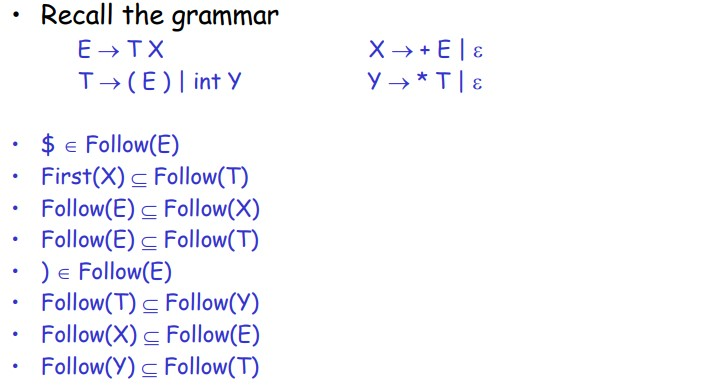
\includegraphics[width=0.8\linewidth]{fig/follow_eg1.jpg}\\
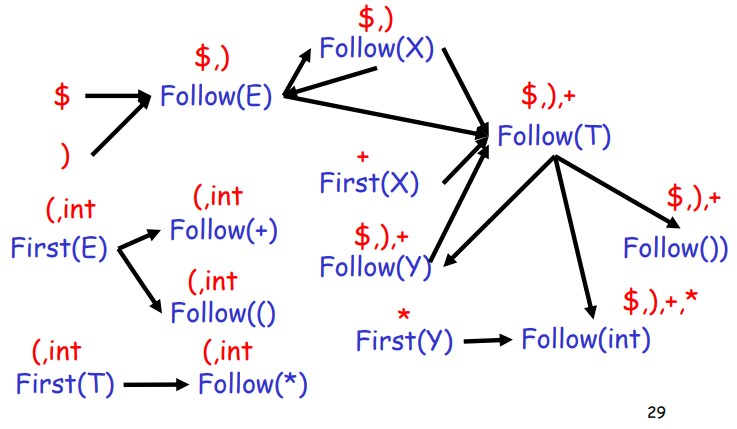
\includegraphics[width=0.8\linewidth]{fig/follow_eg2.jpg}
\end{tabular}
\end{figure}

\subsection{自顶向下分析}
\subsubsection{递归下降}
递归下降语法翻译即从顶层的非终端符号$E$开始,顺序尝试$E$的所有规则,不断回溯遍历,完整例子可见\href{http://web.stanford.edu/class/cs143/lectures/lecture06.pdf}{此文档}。

\begin{algorithm}[H]
\centering
\caption{递归下降(top-down parser)}
\begin{algorithmic}[1]
\State 选择$A$生成式$A\to X_1X_2\cdots X_k$
\For{$i=1$ to $k$}
\If{$X_i$是非终端符号}
\State 调用$X_i()$
\Else\If{$X_i$等于当前的输入符号$a$}
\State 读取下一输入符号
\Else
\State $error()$
\EndIf
\EndIf
\EndFor
\end{algorithmic}
\end{algorithm}

\subsubsection{LL(1)文法}
\begin{definition}[LL(1)文法\protect\footnote{第一个L代表输入字符串从左边开始扫描,第二个L代表得到的推导是最左推导,(1)代表向前看1个输入符号(或单词)}]
语法$G$是LL(1)文法当且仅当对于任意$A\to\alpha\mid\beta$为$G$两个不同的生成式,满足
\begin{enumerate}
	\item $\alpha$和$\beta$不会同时推导出由同一终端符号$a$开始的字符串
	\item $\alpha$和$\beta$中至多一个能获得空字串
	\item 若$\beta\to\epsilon$,则$\alpha$不能推出任何以$FOLLOW(A)$中终端符号开始的字符串;
	同样地,若$\alpha\to\epsilon$,则$\beta$不能推出任何以$FOLLOW(A)$中终端符号开始的字符串
\end{enumerate}
前两个条件等价于\textcolor{red}{$FIRST(\alpha)\cap FIRST(\beta)=\varnothing$},第三个条件等价于若$\epsilon\in FIRST(\beta)$,则\textcolor{red}{$FIRST(\alpha)\cap FOLLOW(A)=\varnothing$},反之同理。
这三个条件的作用都是\textbf{避免在输入符号上冲突}。
\end{definition}
通常没有左递归、无歧义的语法可以是LL(1)。

递归下降在每一步都会有多种生成式的选择,这会导致大量的回溯。
而在LL(1)文法中,每一步都\textbf{只有一种生成式的选择,避免了回溯}。

\begin{example}
经典的二义if-else语法(已提取左因子)
\[\begin{aligned}
S &\to iEtSS'\mid a\\
S' &\to eS\mid\epsilon\\
E &\to b
\end{aligned}\]
可以求得
\[\begin{aligned}
FIRST(S) &= \{i,a\}\\
FIRST(S') &= \{\epsilon,e\}\\
FIRST(E) &= b\\
FOLLOW(S) &= \{\$\} + FIRST(S')-\{\epsilon\}=\{\$,e\}\\
FOLLOW(S') &= \{\$\} + FOLLOW(S) = \{\$,\textcolor{red}{e}\}\\
FOLLOW(E) &= \{\$,t\}
\end{aligned}\]
因为$\epsilon\in FIRST(S'\to\epsilon)$里,而$FIRST(S'\to eS)\cap FOLLOW(S')=\{e\}\ne\varnothing$,所以不是LL(1)文法。
\end{example}

\begin{myalgorithm}[构造LL(1)预测语法表]
对于每一生成式$A\to\alpha$,
\begin{enumerate}
	\item 对于每一终端符号$a\in FIRST(\textcolor{red}{\alpha})$,将$A\to\alpha$添加到$M[A,a]$中。
	\item 若$\epsilon\in FIRST(\textcolor{red}{\alpha})$,则对$b\in FOLLOW(A)$,将$A\to\alpha$添加到$M[A,b]$中($\beta$可以为\$)。
\end{enumerate}
注意是生成式右端。
\end{myalgorithm}

\begin{example}
考虑以下文法
\[\begin{aligned}
E &\to T + E\mid T\\
T &\to int \mid int * T\mid (E)
\end{aligned}\]
提取左因子后即得
\[\begin{aligned}
E &\to TX\\
X &\to +E\mid \epsilon\\
T &\to int\;Y\mid (E)\\
Y &\to *T\mid \epsilon
\end{aligned}\]
$FIRST$集和$FOLLOW$集的推导可见上面的图,注意$FOLLOW(T)$和$FOLLOW(Y)$很容易推漏
\[\begin{array}{rlrl}
FIRST(Y) &=\{*,\epsilon\} & FOLLOW(E) &=\{),\$\}\\
FIRST(T) &=\{int,(\} & FOLLOW(X) &=\{),\$\}\\
FIRST(X) &=\{+,\epsilon\} & FOLLOW(T) &=\{+,),\$\}\\
FIRST(E) &=\{int,(\} & FOLLOW(Y) &=\{+,),\$\}
\end{array}\]
有LL(1)语法表,其中最左列为最左非终端符号,最上行为下一输入符号,表格内容为使用的右端生成式。
\begin{center}
\begin{tabular}{|c|c|c|c|c|c|c|}\hline
 & $int$ & $*$ & $+$ & $($ & $)$ & \$\\\hline
$E$ & $TX$ & & & $TX$ & & \\\hline
$X$ &  &  & $+E$ & & $\epsilon$ & $\epsilon$\\\hline
$T$ & $int\; Y$ & & & $(E)$ & &\\\hline
$Y$ &  & $*T$ & $\epsilon$ & & $\epsilon$ & $\epsilon$\\\hline
\end{tabular}
\end{center}
\end{example}

基于表的预测语法分析,用栈实现。
\begin{algorithm}[H]
\caption{Table-Driven Predictive Parsing}
\begin{algorithmic}[1]
\State \verb'ip=0'
\State \verb'X=stack.top()'
\While {$X\ne\$$}
\If {X == w[ip]}
\State \verb'stack.pop(); ip++;'
\Else \If {X is a terminal or M[X,a]=$\varnothing$}
\State Error()
\Else
\State Output production \verb'M[X,a]'$=X\to Y_1Y_2\cdots Y_k$
\State stack.pop()
\State push $Y_k,Y_{k-1},\ldots,Y_1$ onto the stack
\EndIf
\EndIf
\State \verb'X=stack.top()'
\EndWhile
\If {w[ip] != '\$'}
\State Error()
\EndIf
\end{algorithmic}
\end{algorithm}

\begin{example}
考虑下面语法
\[\begin{array}{lrl}
(1) & E &\to T E'\\
(2) & E' &\to + T E'\mid\epsilon\\
(3) & T &\to F T'\\
(4) & T' &\to * F T'\mid\epsilon\\
(5) & F &\to (E) \mid id
\end{array}\]
计算$FIRST$集
\begin{itemize}
	\item 从终端符号多的开始(5),$FIRST(F)=\{(,id\}$
	\item 向上找含$F$的生成式(3),$FIRST(T)=FIRST(F)$
	\item 向上找含$T$的生成式(1),$FIRST(E)=FIRST(T)$
	\item $FIRST(E')=\{+,\epsilon\}$
	\item $FIRST(T')=\{*,\epsilon\}$
\end{itemize}
计算$FOLLOW$集
\begin{itemize}
	\item 从起始符号开始(1),注意(5)也有$E$,故$FOLLOW(E)=\{),\$\}$
	\item $E'$只出现在$E$的生成式末尾,因此$FOLLOW(E')=FOLLOW(E)=\{),\$\}$
	\item $FOLLOW(T)\subset FIRST(E')=\{+,\epsilon\}$,由于$\epsilon\in FIRST(E')$,故$FOLLOW(T)\subset FOLLOW(E)=\{),\$\}$,即$FOLLOW(T)=\{+,),\$\}$
	\item $FOLLOW(F)\subset FIRST(T')=\{*,\epsilon\}$,由于$\epsilon\in FIRST(T')$,故$FOLLOW(F)\subset FOLLOW(T)=\{+,),\$\}$,即$FOLLOW(F)=\{*,+,),\$\}$
	\item $T'$只出现在$T$的生成式末尾,因此$FOLLOW(T')=FOLLOW(T)=\{*,+,),\$\}$
\end{itemize}
对应有语法预测表
\begin{center}
\begin{tabular}{|c|c|c|c|c|c|c|}\hline
 & $id$ & $+$ & $*$ & $($ & $)$ & \$\\\hline
$E$ & $E\to TE'$ & & & $E\to TE'$ & &\\\hline
$E'$ & & $E'\to +TE'$ & & & \textcolor{red}{$E'\to\epsilon$} & \textcolor{red}{$E'\to\epsilon$}\\\hline
$T$ & $T\to FT'$ & & & $T\to FT'$ & &\\\hline
$T'$ & & $T'\to\epsilon$ & $T'\to*FT'$ & & \textcolor{red}{$T'\to\epsilon$} & \textcolor{red}{$T'\to\epsilon$}\\\hline
$F$ & $F\to id$ & & & $F\to(E)$ & &\\\hline
\end{tabular}
\end{center}
注意上述标红的项为通过第2条规则推导出来的项($\epsilon\in FIRST(\alpha)$)。
\end{example}

\begin{example}
考虑以下文法:
\[\begin{aligned}
S &\to (L) \mid a\\
L &\to L, S \mid S
\end{aligned}\]
\begin{enumerate}
	\item 消除文法的左递归.
	\item 构造文法的LL(1)分析表.
	\item 对于句子$(a, (a, a))$,给出语法分析的详细过程(参照课本228页的图4.21).
\end{enumerate}
\end{example}
\begin{analysis}
\begin{enumerate}
	\item 如下
	\[\begin{aligned}
	S &\to (L)\mid a\\
	L &\to SL'\\
	L' &\to , SL'\mid\epsilon
	\end{aligned}\]
	\item 先求出FIRST集和FOLLOW集(由于文法中存在逗号,故将字符用引号括起来以示区分)
	\[\begin{array}{rlrl}
	FIRST(S) &= \{'(','a'\} & FOLLOW(S) &= \{'\$',')'\}\\
	FIRST(L) &= \{'(','a'\} & FOLLOW(L) &= \{')'\}\\
	FIRST(L') &= \{',',\epsilon\} & FOLLOW(L') &= \{')'\}
	\end{array}\]
	LL(1)分析表如下,其中第一列为非终端符号,第一行为输入符号.
	\begin{center}
	\begin{tabular}{|c|c|c|c|c|c|}\hline
	 & $($ & $)$ & $a$ & $,$ & \$\\\hline
	S & $S\to(L)$ & & $S\to a$ & &\\\hline
	L & $L\to SL'$ & & $L\to SL'$ & &\\\hline
	L' & & $L'\to\epsilon$ & & $L'\to,SL'$ & \\\hline
	\end{tabular}
	\end{center}
	\item 语法分析过程如下
	\begin{center}
	\begin{tabular}{|l|r|r|l|}\hline
	Matched & Stack & Input & Action\\\hline
	 & $S\$$ & $(a,(a,a))\$$ & \\\hline
	 & $(L)\$$ & $(a,(a,a))\$$ & output $S\to (L)$\\\hline
	$($ & $L)\$$ & $a,(a,a))\$$ & \\\hline
	$($ & $SL')\$$ & $a,(a,a))\$$ & output $L\to SL'$\\\hline
	$($ & $aL')\$$ & $a,(a,a))\$$ & output $S\to a$\\\hline
	$(a$ & $L')\$$ & $,(a,a))\$$ & \\\hline
	$(a$ & $,SL')\$$ & $,(a,a))\$$ & output $L'\to ,SL'$\\\hline
	$(a,$ & $SL')\$$ & $(a,a))\$$ & \\\hline
	$(a,$ & $(L)L')\$$ & $(a,a))\$$ & output $S\to (L)$\\\hline
	$(a,($ & $L)L')\$$ & $a,a))\$$ & \\\hline
	$(a,($ & $SL')L')\$$ & $a,a))\$$ & output $L\to SL'$\\\hline
	$(a,($ & $aL')L')\$$ & $a,a))\$$ & output $S\to a$\\\hline
	$(a,(a$ & $L')L')\$$ & $,a))\$$ & \\\hline
	$(a,(a$ & $,SL')L')\$$ & $,a))\$$ & output $L'\to,SL'$\\\hline
	$(a,(a,$ & $SL')L')\$$ & $a))\$$ & \\\hline
	$(a,(a,$ & $aL')L')\$$ & $a))\$$ & output $S\to a$\\\hline
	$(a,(a,a$ & $L')L')\$$ & $))\$$ & \\\hline
	$(a,(a,a$ & $)L')\$$ & $))\$$ & output $L'\to\epsilon$\\\hline
	$(a,(a,a)$ & $L')\$$ & $)\$$ & \\\hline
	$(a,(a,a)$ & $)\$$ & $)\$$ & output $L'\to\epsilon$\\\hline
	$(a,(a,a))$ & $\$$ & $\$$ & \\\hline
	\end{tabular}
	\end{center}
\end{enumerate}
\end{analysis}

\subsection{自底向上分析}
自底向上的语法分析采用两种动作:
\begin{itemize}
\item 移进(shift):将\verb'|'向右移动一格
\[ABC\mid xyz\implies ABCx\mid yz\]
\item 规约(reduce):在字符串右侧逆向应用生成式
\[Cbxy\mid ijk\implies CbA\mid ijk\]
\end{itemize}

\begin{figure}[H]
\centering
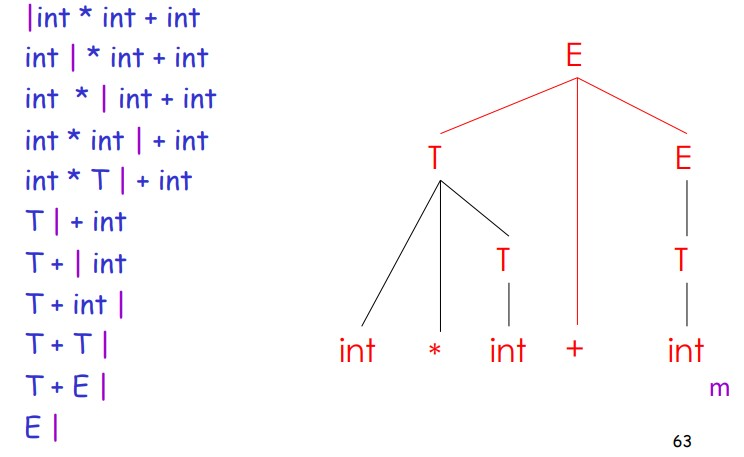
\includegraphics[width=0.8\linewidth]{fig/shift-reduce.jpg}
\end{figure}
移进将终端符号移入栈中,规约将生成式的右端符号弹出,将生成式的左端\textbf{非终端}符号推入。

\begin{definition}[句柄(handle)]
A handle is a string that can be \textbf{reduced} and also allows further reductions back to the start symbol.
可以理解为当前正在处理的token,用于\textbf{规约}(生成式的右端)而不是移进。
\end{definition}

\begin{definition}[活前缀(viable prefix)]
$\alpha$是活前缀若存在$\omega$使得$\alpha\mid\omega$是移进-规约语法分析器的状态。
\end{definition}

LR分析是最通用的\textbf{非回溯}移进-规约语法解析方法,难点在于构建分析表太过麻烦,但Yacc等工具可辅助构建。

\subsubsection{LR(0)语法}
为构建规范(canoical)LR(0)项,\textbf{定义增量语法$G'$有生成式$S'\to S$},其中$S$为原语法$G$的开始符号。
这个生成式用于告知parser接受(accept)输入并停止解析,即接受仅发生在要对$S'\to S$进行规约的时候。

\begin{definition}[CLOSURE]
若$I$为语法$G$项的集合,则$CLOSURE(I)$为从$I$中构造出项的集合:
\begin{enumerate}
	\item 初始时,在$I$中的每一项都会被加到$CLOSURE(I)$中
	\item 若$A\to\alpha\cdot B\beta$在$CLOSURE(I)$中且$B\to\beta$是一个生成式,则将项$B\to\cdot\gamma$加入到$CLOSURE(I)$中;重复使用此规则,直至没有新项可以被加入
\end{enumerate}
\end{definition}
\begin{definition}[GOTO]
$I$是项的集合,$X$为输入符号,$GOTO(I,X)$为所有项$[A\to\alpha X\cdot\beta]$的闭包使得$[A\to\alpha\cdot X\beta]$在$I$中
\end{definition}

\begin{definition}[核项(kernel item)]
初始项$S'\to\cdot S$及所有$\cdot$不在左端的项称为核项,
除了初始项外所有$\cdot$在左端的项称为非核项(即那些新加入闭包的项)
\end{definition}

\begin{definition}[LR(0)语法]
栈包含$\alpha$,下一输入是$t$,DFA在输入$\alpha$上终止在状态$s$
\begin{itemize}
	\item 当$s$包含$X\to\beta$的项时进行规约(没有得移进就规约,自动机无对应符号出边)
	\item 当$s$包含$X\to\beta.t\omega$的项时移进
\end{itemize}
\end{definition}

LR(0)可能存在以下两种冲突:
\begin{itemize}
	\item 规约-规约冲突:$X\to\beta.$且$Y\to\omega.$
	\item 移进-规约冲突:$X\to\beta.$且$Y\to\omega.t\delta$
\end{itemize}

\subsubsection{SLR分析}
SLR(simple left-to-right scan)\footnote{或SLR(1)分析,通常省略(1)。用的是LR(0)项,但是在语法分析时才前看1个输入符号。}用启发式算法提升了LR(0)移进规约的效率,减少冲突。
\begin{definition}[SLR(1)语法]
栈包含$\alpha$,下一输入是$t$,DFA在输入$\alpha$上停在状态$s$
\begin{itemize}
	\item 当$s$包含$X\to\beta$的项且\textcolor{red}{$t\in FOLLOW(X)$}时进行$X\to\beta$规约
	\item 当$s$包含$X\to\beta.t\omega$的项时移进
\end{itemize}
\end{definition}

\begin{myalgorithm}[SLR(1)分析表]
构造$\mathcal{C}=\{I_0,I_1,\ldots,I_n\}$为LR(0)项的集合$G'$
\begin{enumerate}
	\item 若$[A\to\alpha\cdot a \beta]\in I_i$且$GOTO(I_i,a)=I_j$,则设$ACTION[i,a]$为移进$j$,
	\item 若$[A\to\alpha\cdot]\in I_i$,则$\forall a\in FOLLOW(A)$,设$ACTION[i,a]$为规约$A\to\alpha$
	\item 若$[S'\to S\cdot]\in I_i$,则设$ACTION[i,\$]$为接受(ACC)
\end{enumerate}
若上述有冲突的动作,则该文法不是SLR(1)的。

依照分析表可以得到语法分析的算法
\begin{itemize}
	\item 若$ACTION[s,a]$为移进$t$,则将$t$\textbf{推入}栈中
	\item 若$ACTION[s,a]$为\textbf{规约$A\to\beta$},则将\textcolor{red}{$|\beta|$个}符号从栈顶\textbf{弹出},令$t$为\textbf{栈顶符号},\textbf{将$GOTO[t,A]$推入栈中},输出规约$A\to\beta$
	\item 若$ACTION[s,a]=acc$,则语法解析结束
\end{itemize}
\end{myalgorithm}

\begin{example}
考虑以下文法:
\[\begin{array}{rrll}
(1) & E &\to & E+T\\
(2) & E &\to & T\\
(3) & T &\to & TF\\
(4) & T &\to & F\\
(5) & F &\to & F^*\\
(6) & F &\to & a\\
(7) & F &\to & b
\end{array}\]
\begin{enumerate}
	\item 写出每个非终端符号的FIRST集和FOLLOW集.
	\item 构造识别这一文法所有活前缀(viable prefixes)的LR(0)自动机(参照课本4.6.2节图4.31).
	\item 构造这一文法的SLR分析表(参照课本4.6.3节图4.37).
	\item 给出SLR分析器识别输入串$a+ab^*$的过程(参照课本4.6.4节图4.38)
\end{enumerate}
\end{example}
\begin{analysis}
\begin{enumerate}
	\item $FIRST$集和$FOLLOW$集如下
	\[\begin{array}{rlrl}
	FIRST(E) &= \{a,b\} & FOLLOW(E) &=\{\$,+\}\\
	FIRST(T) &= \{a,b\} & FOLLOW(T) &=\{\$,+,a,b\}\\
	FIRST(F) &= \{a,b\} & FOLLOW(F) &=\{\$,+,*,a,b\}\\
	\end{array}\]
	\item 构造增广语法$E'\to E$,并得到LR(0)自动机如下
	\begin{figure}[H]
	\centering
	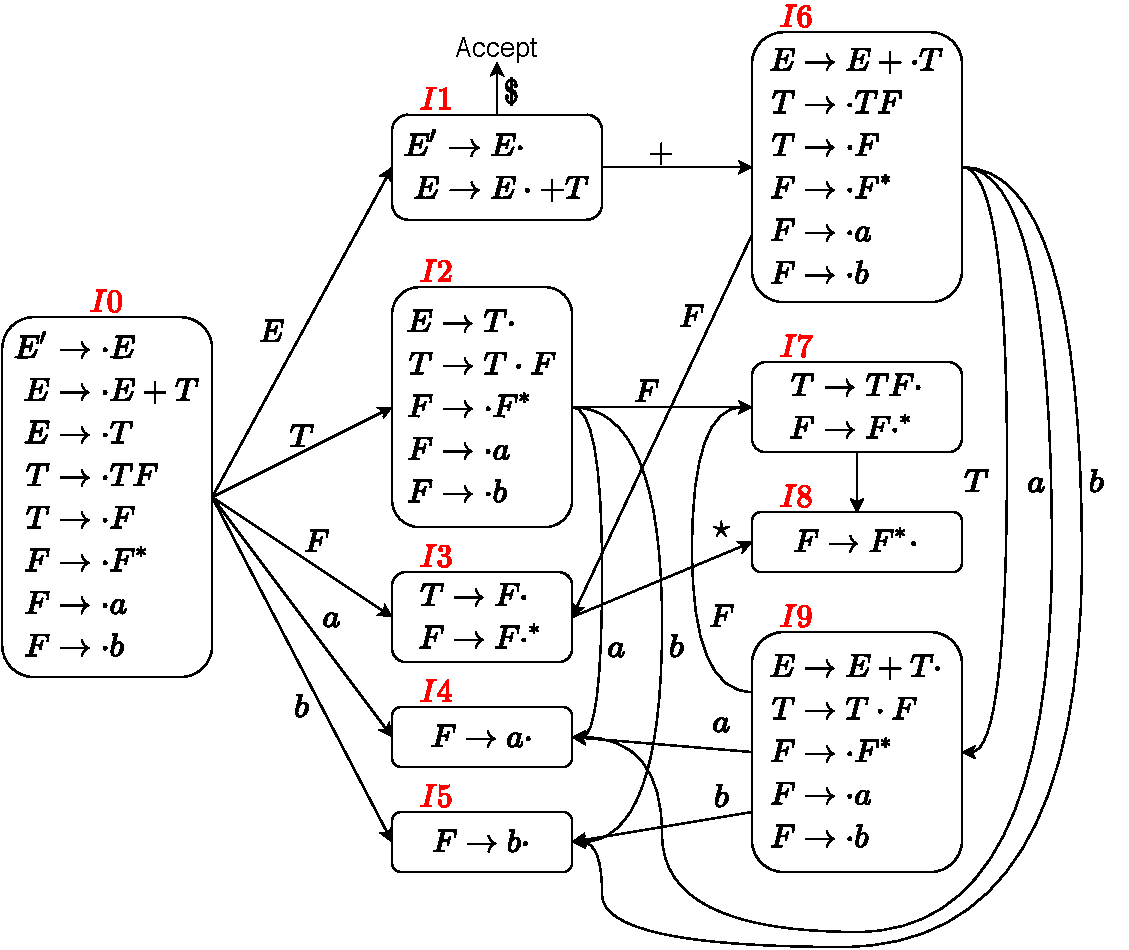
\includegraphics[width=0.8\linewidth]{fig/T06.pdf}
	\end{figure}
	\item 依据上述两问结果,可构造SLR分析表如下(s后面的数字为DFA状态编号,r后面的数字为生成式的编号)
	\begin{center}
	\begin{tabular}{|c|ccccc|ccc|}\hline
	\multirow{2}{*}{STATE} & \multicolumn{5}{c|}{ACTION} & \multicolumn{3}{c|}{GOTO}\\\cline{2-9}
	  & a  & b  & +  & *  & \$  & E & T & F \\\hline
	0 & s4 & s5 &    &    &     & 1 & 2 & 3 \\\hline
	1 &    &    & s6 &    & ACC &   &   &   \\\hline
	2 & s4 & s5 & r2 &    & r2  &   &   & 7 \\\hline
	3 & r4 & r4 & r4 & s8 & r4  &   &   &   \\\hline
	4 & r6 & r6 & r6 & r6 & r6  &   &   &   \\\hline
	5 & r7 & r7 & r7 & r7 & r7  &   &   &   \\\hline
	6 & s4 & s5 &    &    &     &   & 9 & 3 \\\hline
	7 & r3 & r3 & r3 & s8 & r3  &   &   &   \\\hline
	8 & r5 & r5 & r5 & r5 & r5  &   &   &   \\\hline
	9 & s4 & s5 & r1 &    & r1  &   &   & 7 \\\hline
	\end{tabular}
	\end{center}
	\item 依上述ACTION-GOTO表,可得以下过程
	\begin{center}
	\begin{tabular}{|r|l|l|r|l|}\hline
		& STACK & SYMBOLS & INPUT      & ACTION\\\hline
	(1) & 0     &         & $a+ab^*\$$ & $[0,a]s4$\\\hline
	(2) & 04    & $a$     & $+ab^*\$$  & $[4,a]r6\;F\to a$, $[0,F]s3$\\\hline
	(3) & 03    & $F$     & $+ab^*\$$  & $[3,+]r4\;T\to F$, $[0,T]s2$\\\hline
	(4) & 02    & $T$     & $+ab^*\$$  & $[2,+]r2\;E\to T$, $[0,E]s1$\\\hline
	(5) & 01    & $E$     & $+ab^*\$$  & $[1,+]s6$\\\hline
	(6) & 016    & $E+$     & $ab^*\$$  & $[6,a]s4$\\\hline
	(7) & 0164    & $E+a$     & $b^*\$$  & $[4,b]r6\;F\to a$, $[6,F]s3$\\\hline
	(8) & 0163    & $E+F$     & $b^*\$$  & $[3,b]r4\;T\to F$, $[6,T]s9$\\\hline
	(9) & 0169    & $E+T$     & $b^*\$$  & $[9,b]s5$\\\hline
	(10) & 01695  & $E+Tb$    & ${}^*\$$ & $[5,*]r7\;F\to b$, $[9,F]s7$\\\hline
	(11) & 01697  & $E+TF$    & ${}^*\$$ & $[7,*]s8$\\\hline
	(12) & 016978 & $E+TF^*$    & $\$$ & $[8,\$]r5\;F\to F^*$, $[\textcolor{red}{9},F]s7$\\\hline
	(13) & 01697  & $E+TF$    & $\$$ & $[7,\$]r3\;T\to TF$, $[\textcolor{red}{6},T]s9$\\\hline
	(14) & 0169   & $E+T$     & $\$$ & $[9,\$]r1\;E\to E+T$, $[\textcolor{red}{0},E]s1$\\\hline
	(15) & 01     & $E$     & $\$$ & $[1,\$]ACC$\\\hline
	\end{tabular}
	\end{center}
\end{enumerate}
\end{analysis}

\begin{example}
下面的文法并非SLR(1)
\[\begin{aligned}
S &\to L=R\mid R\\
L &\to *R\mid id\\
R &\to L
\end{aligned}\]
对于$I_2$项:
\[\begin{aligned}
S &\to L\cdot=R\\
R &\to L\cdot
\end{aligned}\]
有$ACTION[2,=]$是移进,但$FOLLOW(R)=\{\$,=\}$又会导致在$=$上进行规约,故移进-规约冲突,该文法不是SLR(1)的
\end{example}

\subsubsection{LR(1)语法}
\begin{definition}[LR(1)项]
$[A\to\alpha\cdot\beta,a]$,其中$A\to\alpha\cdot\beta$为该项的核(core),$A\to\alpha\beta$为生成式,$a$是终端符号或\$,1指项中第二个元素的长度,$a$也被称为前看(lookahead)。
只有当LR(1)项有$[A\to\alpha\cdot,a]$的形式,\textbf{且下一输入符号为$a$时,才会用$A\to\alpha$进行规约}(这在构造解析表时会用到)。
$a$总会是$FOLLOW(A)$的子集,但往往是真子集。
\end{definition}

\begin{myalgorithm}[计算$CLOSURE(I)$]
对于每一$[A\to\alpha\cdot B\beta,a]\in I$,每一$G'$中的生成式$B\to\gamma$,$\forall b\in FIRST(\textcolor{red}{\beta a})$,将$[B\to\cdot\gamma,b]$加入$I$中。

初始化$\mathcal{C}=\{CLOSURE(\{[S'\to\cdot S,\$]\})\}$。
\end{myalgorithm}
\begin{example}
考虑下面的增量语法
\[\begin{array}{rrl}
(1) & S' &\to S\\
(2) & S &\to C C\\
(3) & C &\to c C\mid d
\end{array}\]
有$FIRST(C)=\{c,d\}$,可以构造得下面的LR(1)自动机。
以$[S\to\cdot CC,\$]$为例,考虑$FIRST(C\$)=\{c,d\}$,故闭包会新增四项$[C\to\cdot cC,c]$、$[C\to\cdot cC,d]$、$[C\to\cdot d,c]$、$[C\to\cdot d,d]$。
\begin{figure}[H]
\centering
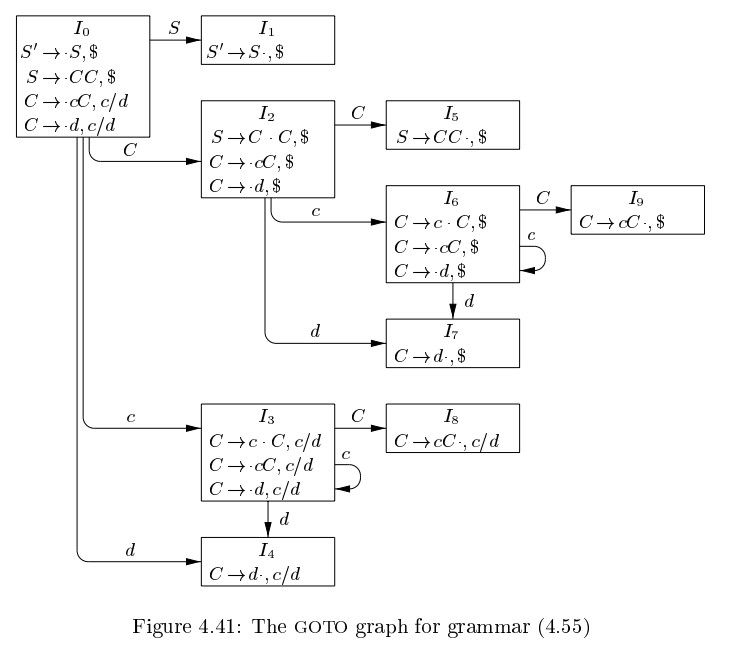
\includegraphics[width=0.8\linewidth]{fig/LR1-eg.jpg}
\end{figure}
类似地有规范LR(1)解析表
\begin{center}
\begin{tabular}{|c|c|c|c|c|c|}\hline
  & c  & d  & \$  & S & C \\\hline
0 & s3 & s4 &     & 1 & 2 \\\hline
1 &    &    & acc &   &   \\\hline
2 & s6 & s7 &     &   & 5 \\\hline
3 & s3 & s4 &     &   & 8 \\\hline
4 & r3 & r3 &     &   &   \\\hline
5 &    &    & r1  &   &   \\\hline
6 & s6 & s7 &     &   & 9 \\\hline
7 &    &    & r3  &   &   \\\hline
8 & r2 & r2 &     &   &   \\\hline
9 &    &    & r2  &   &   \\\hline
\end{tabular}
\end{center}
\end{example}

LR(0)=SLR(1)的表项较少,但LR(1)的表项就指数级上涨。

\subsubsection{LALR分析}
LALR(Lookahead LR)在实践中很常用,表大小通常远小于规范LR表。
核心思想是将LR(1)中具有\textbf{相同核}的表项合并。

\begin{example}
将上面例子中的$I_3$和$I_6$合并得到
\[\begin{aligned}
C &\to c\cdot C, c/d/\$\\
C &\to \cdot cC, c/d/\$\\
C &\to \cdot d, c/d/\$
\end{aligned}\]
$I_4$和$I_7$合并得到
\[\begin{aligned}
C &\to d\cdot, c/d/\$
\end{aligned}\]
$I_8$和$I_9$合并得到
\[\begin{aligned}
C &\to cC\cdot, c/d/\$
\end{aligned}\]
进而有LALR解析表
\begin{center}
\begin{tabular}{|c|c|c|c|c|c|}\hline
   & c   & d   & \$  & S & C \\\hline
0  & s36 & s47 &     & 1 & 2 \\\hline
1  &     &     & acc &   &   \\\hline
2  & s36 & s47 &     &   & 5 \\\hline
36 & s36 & s47 &     &   & 89\\\hline
47 & r3  & r3  & r3  &   &   \\\hline
5  &     &     & r1  &   &   \\\hline
89 & r2  & r2  & r2  &   &   \\\hline
\end{tabular}
\end{center}
\end{example}

合并LR(1)项不会导致新的移进-规约冲突,但可能会产生新的\textbf{规约-规约冲突}。

\begin{example}
证明下列文法
\[\begin{aligned}
S &\to Aa \mid bAc \mid dc \mid bda\\
A &\to d
\end{aligned}\]
是LALR(1)文法但不是SLR(1)文法.
\end{example}
\begin{analysis}
构造增广文法$S'\to\cdot S$,$FIRST(\epsilon\$)=\$$,$FIRST(a\$)=a$,可以得到$I_0$。
\begin{figure}[H]
\centering
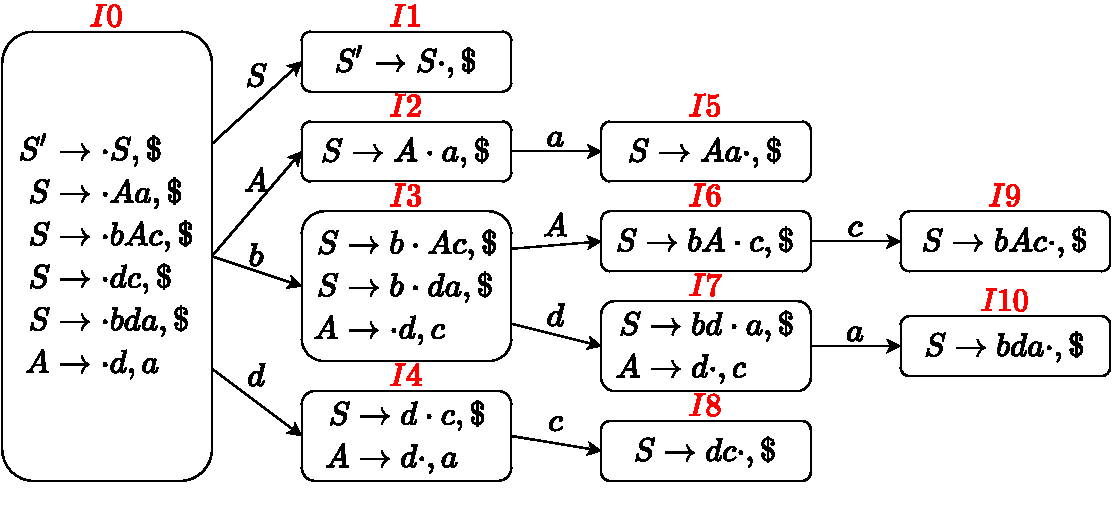
\includegraphics[width=0.8\linewidth]{fig/T07-1.pdf}
\end{figure}
由上图知,没有相同核心(core)的状态,因此不需要合并,从而LALR分析表不冲突,该文法是LALR(1)文法。

又有$FOLLOW(A)=\{a,c\}$,考虑图中的状态$I4$,当输入符号为$c$时,$c\in FOLLOW(A)$,既有移进$S\to d\cdot c$,又有归约$S\to d\cdot$,因此SLR分析表有冲突,该文法不是SLR(1)文法。
\end{analysis}
\begin{example}
证明下列文法
\[\begin{aligned}
S &\to Aa \mid bAc \mid Bc \mid bBa\\
A &\to d\\
B &\to d
\end{aligned}\]
是LR(1)文法但不是LALR(1)文法.
\end{example}
\begin{analysis}
构造增广文法$S'\to\cdot S$,$FIRST(a\$)=a$,$FIRST(c\$)=c$,可以得到状态$I_0$。
\begin{figure}[H]
\centering
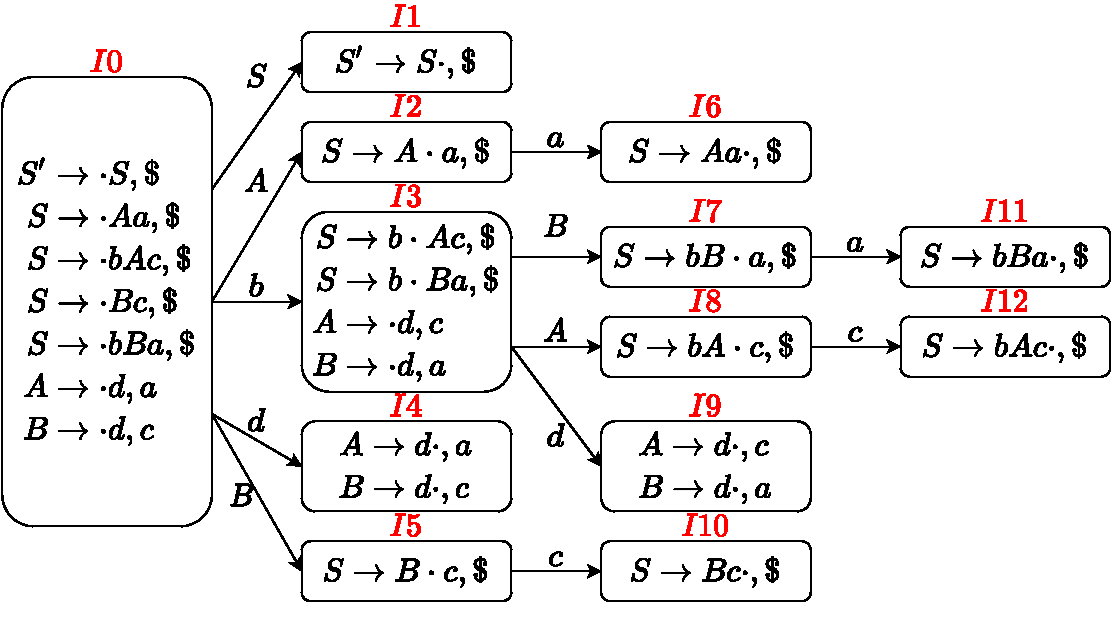
\includegraphics[width=0.8\linewidth]{fig/T07-2.pdf}
\end{figure}
由上面的DFA知LR分析表没有冲突,因此该文法是LR(1)文法。

但如果将图中相同核心的状态$I4$和$I9$合并,会有
\[\begin{aligned}
A &\to d\cdot,a/c\\
B &\to d\cdot,a/c
\end{aligned}\]
即出现了规约-规约冲突,因此该文法不是LALR(1)文法。
\end{analysis}

可以在解析表(parsing table)层面来解决语法的二义性,即选择移进/规约的特定操作。

\subsection{语法制导翻译}
抽象语法树(Abstract Syntax Trees, AST)是将原本语法树中冗余的成分给去除,比如左右括号原本都是各自一个结点,但在AST中不会呈现。

语法制导翻译(syntax-directed translation)给语法符号提供了属性(attribute),给生成式提供了动作(action)。
\begin{example}
对下列语法进行求值
\[E\to int\mid E+E\mid (E)\]
有语法制导定义
\begin{center}
\begin{tabular}{ll}
$E\to int$ & $E.val=int.val$\\
$E\to E_1+E_2$ & $E.val=E_1.val+E_2.val$\\
$E\to (E_1)$ & $E.val=E_1.val$
\end{tabular}
\end{center}
\end{example}

可以在AST上标注(annotate)两种属性:
\begin{itemize}
\item 继承属性(inherited):从语法树的父亲或兄弟中计算得到
\item 综合属性(synthesized):从后代计算得到
\end{itemize}

\forestset{
sn edges/.style={for tree={edge={-}}}
}

\begin{example}
考虑以下语法制导定义:
\begin{center}
\begin{tabular}{|l|l|}\hline
\multicolumn{1}{|c|}{语法规则} & \multicolumn{1}{c|}{语义规则}\\\hline
$S \to ABCD$ & $S.val = A.val + B.val + C.val + D.val$\\\hline
$A \to gBa$ & $A.val = B.val * 5$\\\hline
$B \to B_1b$ & $B.val = B_1.val * 2$\\\hline
$B \to b$ & $B.val = 2$\\\hline
$C \to C_1c$ & $C.val = C_1.val * 3$\\\hline
$C \to c$ & $C.val = 3$\\\hline
$D \to d$ & $D.val = 1$\\\hline
\end{tabular}
\end{center}
对于输入串$gbbabbccd$构造带注释的分析树(annotated parse tree).
\end{example}
\begin{analysis}
带注释的分析树如下
\begin{center}
\begin{forest}
sn edges
[{$S.val=20+4+9+1=34$}
	[{$A.val=4*5=20$}
		[{$\mathbf{g}$}]
		[{$B.val=2*2=4$}
			[{$B.val=2$}
				[{$\mathbf{b}$}]
			]
			[{$\mathbf{b}$}]
		]
		[{$\mathbf{a}$}]
	]
	[{$B.val=2*2=4$}
		[{$B.val=2$}
			[{$\mathbf{b}$}]
		]
		[{$\mathbf{b}$}]
	]
	[{$C.val=3*3=9$}
		[{$C.val=3$}
			[{$\mathbf{c}$}]
		]
		[{$\mathbf{c}$}]
	]
	[{$D.val=1$}
		[{$\mathbf{d}$}]
	]
]
\end{forest}
\end{center}
\end{analysis}

\begin{example}
下列文法定义了二进制整数的语法规则
\[\begin{aligned}
N &\to SL\\
L &\to LB\mid B\\
S &\to +\mid -\\
B &\to 0\mid 1
\end{aligned}\]
给出语法制导定义,求出该二进制整数的十进制值,存在综合属性\verb'val'中
\begin{center}
\begin{tabular}{|c|l|l|}\hline
序号 & 生成式 & 语义规则\\\hline
1 & $N\to SL$ & $N.val=S.sign*L.val$\\\hline
2 & $L\to L_1 B$ & $L.val=L_1.val*2+B.val$\\\hline
3 & $L\to B$ & $L.val=B.val$\\\hline
4 & $S\to +$ & $S.sign=1$\\\hline
5 & $S\to -$ & $S.sign=-1$\\\hline
6 & $B\to 0$ & $B.val=0$\\\hline
7 & $B\to 1$ & $B.val=1$\\\hline
\end{tabular}
\end{center}
\end{example}

扩展文法:
\[\begin{array}{rll}
expr &\to expr_1 + term & \{print('+')\}\\
expr &\to expr_1 - term & \{print('-')\}\\
expr &\to term & \\
term &\to 0    & \{print('0')\}\\
term &\to 1    & \{print('1')\}\\
     &\vdots   & \\
term &\to 9    & \{print('9')\}\\
\end{array}\]
大括号中的语句称为动作(action),这一系列产生式称为翻译模式(translation scheme)。

将动作视为产生式右端的一部分,则可得到扩展的语法树。
对语法分析树做先序遍历,则可以得到后缀表达式。

\subsection{总结}
语法分析分为自顶向下和自底向上两大类,自顶向下是从开始符号出发,根据产生式规则\textbf{推导}给定的句子;自底向上则是由给定的句子\textbf{规约}到文法的开始符号。

其中LL(1)是自顶向下的分析法,LR(0)、SLR(1)、LR(1)、LALR(1)是自底向上的分析法。
\begin{center}
\begin{tabular}{|c|c|c|}\\\hline
文法 & 文法要求 & 构造分析表 \\\hline
LL(1) & 生成式首符号不能相同 & 将生成式加到首符号项上\\\hline
LR(0) & LR(0)自动机无冲突 & \\\hline
SLR(1) & 下一输入$a\in FOLLOW(X)$时进行规约 & ACTION-GOTO表同左\\\hline
LR(1) & 用$FIRST(\beta a)$确定前看项无冲突 & 下一输入为$a$才规约$[A\to\alpha\cdot,a]$\\\hline
LALR(1) & 将LR(1)相同核项合并无冲突 & 同上\\\hline
\end{tabular}
\end{center}

% LL(1) Matched Stack Input Action
% LR(0) Stack Symbols Input Action

文法处理能力:LR(0) $<$ SLR(1) $<$ LALR(1) $<$ LR(1)

\end{document}